\newpage
%%%%%%%%%%%%%%%%%%%%%%%%%%%%%%%%%%%%%%%%%%%%%%%%%%%%%%%%%%%%%%%%%%%%%%%%%%%%%%%
\section{Week 5}
%%%%%%%%%%%%%%%%%%%%%%%%%%%%%%%%%%%%%%%%%%%%%%%%%%%%%%%%%%%%%%%%%%%%%%%%%%%%%%%
\subsection*{I can't be asked}
\begin{itemize}
    \item I am too lazy to summarize my shitty git commits from the 13 til now
        (the 31st).
    \item Enjoy Mr. Incredible Uncanny 4 instead:
    \begin{figure}[ht]
        \centering
        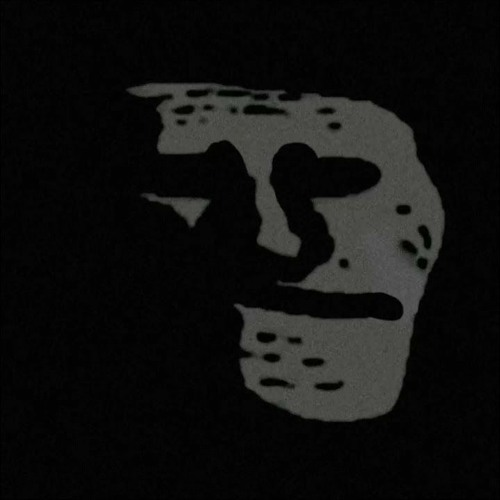
\includegraphics[width=6cm]{uncanny4}
        \captionsetup{labelfont=bf, textfont=it}
        \caption{oooooooooooooooooooo}
        \label{fig:uncanny4}
    \end{figure}
    \item Right, now I've added a few things:
        \begin{itemize}
            \item custom link style and formatting in casts 
            \item render images in casts
            \item sign in with farcaster (doesn't do much else yet)
            \item link to view cast on warpcast 
        \end{itemize}
    \item I suppose I should add reaction data and stuff now.
    \item I'm avoiding the actual hard tech of having the LLM not hallicinate.
        I'm thinking of having a writers room where my proprietary spagetti code
        strips out the things that don't make logical sense from the summary
        from the LLM.
\end{itemize}
